\documentclass[mstat,12pt]{unswthesis}

\usepackage{color}
\usepackage{fancyvrb}
\newcommand{\VerbBar}{|}
\newcommand{\VERB}{\Verb[commandchars=\\\{\}]}
\DefineVerbatimEnvironment{Highlighting}{Verbatim}{commandchars=\\\{\}}
% Add ',fontsize=\small' for more characters per line
\usepackage{framed}
\definecolor{shadecolor}{RGB}{248,248,248}
\newenvironment{Shaded}{\begin{snugshade}}{\end{snugshade}}
\newcommand{\AlertTok}[1]{\textcolor[rgb]{0.94,0.16,0.16}{#1}}
\newcommand{\AnnotationTok}[1]{\textcolor[rgb]{0.56,0.35,0.01}{\textbf{\textit{#1}}}}
\newcommand{\AttributeTok}[1]{\textcolor[rgb]{0.13,0.29,0.53}{#1}}
\newcommand{\BaseNTok}[1]{\textcolor[rgb]{0.00,0.00,0.81}{#1}}
\newcommand{\BuiltInTok}[1]{#1}
\newcommand{\CharTok}[1]{\textcolor[rgb]{0.31,0.60,0.02}{#1}}
\newcommand{\CommentTok}[1]{\textcolor[rgb]{0.56,0.35,0.01}{\textit{#1}}}
\newcommand{\CommentVarTok}[1]{\textcolor[rgb]{0.56,0.35,0.01}{\textbf{\textit{#1}}}}
\newcommand{\ConstantTok}[1]{\textcolor[rgb]{0.56,0.35,0.01}{#1}}
\newcommand{\ControlFlowTok}[1]{\textcolor[rgb]{0.13,0.29,0.53}{\textbf{#1}}}
\newcommand{\DataTypeTok}[1]{\textcolor[rgb]{0.13,0.29,0.53}{#1}}
\newcommand{\DecValTok}[1]{\textcolor[rgb]{0.00,0.00,0.81}{#1}}
\newcommand{\DocumentationTok}[1]{\textcolor[rgb]{0.56,0.35,0.01}{\textbf{\textit{#1}}}}
\newcommand{\ErrorTok}[1]{\textcolor[rgb]{0.64,0.00,0.00}{\textbf{#1}}}
\newcommand{\ExtensionTok}[1]{#1}
\newcommand{\FloatTok}[1]{\textcolor[rgb]{0.00,0.00,0.81}{#1}}
\newcommand{\FunctionTok}[1]{\textcolor[rgb]{0.13,0.29,0.53}{\textbf{#1}}}
\newcommand{\ImportTok}[1]{#1}
\newcommand{\InformationTok}[1]{\textcolor[rgb]{0.56,0.35,0.01}{\textbf{\textit{#1}}}}
\newcommand{\KeywordTok}[1]{\textcolor[rgb]{0.13,0.29,0.53}{\textbf{#1}}}
\newcommand{\NormalTok}[1]{#1}
\newcommand{\OperatorTok}[1]{\textcolor[rgb]{0.81,0.36,0.00}{\textbf{#1}}}
\newcommand{\OtherTok}[1]{\textcolor[rgb]{0.56,0.35,0.01}{#1}}
\newcommand{\PreprocessorTok}[1]{\textcolor[rgb]{0.56,0.35,0.01}{\textit{#1}}}
\newcommand{\RegionMarkerTok}[1]{#1}
\newcommand{\SpecialCharTok}[1]{\textcolor[rgb]{0.81,0.36,0.00}{\textbf{#1}}}
\newcommand{\SpecialStringTok}[1]{\textcolor[rgb]{0.31,0.60,0.02}{#1}}
\newcommand{\StringTok}[1]{\textcolor[rgb]{0.31,0.60,0.02}{#1}}
\newcommand{\VariableTok}[1]{\textcolor[rgb]{0.00,0.00,0.00}{#1}}
\newcommand{\VerbatimStringTok}[1]{\textcolor[rgb]{0.31,0.60,0.02}{#1}}
\newcommand{\WarningTok}[1]{\textcolor[rgb]{0.56,0.35,0.01}{\textbf{\textit{#1}}}}


%%%%%%%%%%%%%%%%%%%%%%%%%%%%%%%%%%%%%%%%%%%%%%%%%%%%%%%%%%%%%%%%%%
% 
% OK...Now we get to some actual input.  The first part sets up
% the title etc that will appear on the front page
%
%%%%%%%%%%%%%%%%%%%%%%%%%%%%%%%%%%%%%%%%%%%%%%%%%%%%%%%%%%%%%%%%%

\title{Capstone Project by Team 3\\[0.5cm]A Data Science Approach to
Forecast Short-term Electricity Demand in NSW}

\authornameonly{Karim Adham (z5468227), Rishantha Rajakaruna
(z5441528), Rushmila Islam (z5456038) }

\author{\Authornameonly}

\copyrightfalse
\figurespagefalse
\tablespagefalse

%%%%%%%%%%%%%%%%%%%%%%%%%%%%%%%%%%%%%%%%%%%%%%%%%%%%%%%%%%%%%%%%%
%
%  And now the document begins
%  The \beforepreface and \afterpreface commands puts the
%  contents page etc in
%
%%%%%%%%%%%%%%%%%%%%%%%%%%%%%%%%%%%%%%%%%%%%%%%%%%%%%%%%%%%%%%%%%%


%%%%%%%%%%%%%%%%%%%%%%%%%%%%%%%%%%%%%%%%%%%%%%%%%%%%%%%%%%%%%%%%%%%%%%%
%
%  A small sample UNSW Coursework Masters thesis file.
%  Any questions to Ian Doust i.doust@unsw.edu.au and/or Gery Geenens ggeenens@unsw.edu.au
%
%%%%%%%%%%%%%%%%%%%%%%%%%%%%%%%%%%%%%%%%%%%%%%%%%%%%%%%%%%%%%%%%%%%%%%%
%
%  The first part pulls in a UNSW Thesis class file.  This one is
%  slightly nonstandard and has been set up to do a couple of
%  things automatically
%
 
%%%%%%%%%%%%%%%%%
%% Precisely one of the next four lines should be uncommented.
%% Choose the one which matches your degree, uncomment it, and comment out the other two!
%\documentclass[mfin,12pt]{unswthesis}    %%  For Master of Financial Mathematics 
%\documentclass[mmath,12pt]{unswthesis}   %%  For Master of Mathematics
%\documentclass[mstat,12pt]{unswthesis}  %%  For Master of Statistics
%%%%%%%%%%%%%%%%%



\linespread{1}
\usepackage{amsfonts}
\usepackage{amssymb}
\usepackage{amsthm}
\usepackage{latexsym,amsmath}
\usepackage{graphicx}
\usepackage{afterpage}
\usepackage[colorlinks]{hyperref}
 \hypersetup{
     colorlinks=true,
     linkcolor=blue,
     filecolor=blue,
     citecolor= black,      
     urlcolor=cyan,
     }
\usepackage{textcomp}
\usepackage{longtable}
\usepackage{booktabs}
\usepackage{float}

%%%%%%%%%%%%%%%%%%%%%%%%%%%%%%%%%%%%%%%%%%%%%%%%%%%%%%%%%%%%%%%%%
%
%  The following are some simple LaTeX macros to give some
%  commonly used letters in funny fonts. You may need more or less of
%  these
%
\newcommand{\R}{\mathbb{R}}
\newcommand{\Q}{\mathbb{Q}}
\newcommand{\C}{\mathbb{C}}
\newcommand{\N}{\mathbb{N}}
\newcommand{\F}{\mathbb{F}}
\newcommand{\PP}{\mathbb{P}}
\newcommand{\T}{\mathbb{T}}
\newcommand{\Z}{\mathbb{Z}}
\newcommand{\B}{\mathfrak{B}}
\newcommand{\BB}{\mathcal{B}}
\newcommand{\M}{\mathfrak{M}}
\newcommand{\X}{\mathfrak{X}}
\newcommand{\Y}{\mathfrak{Y}}
\newcommand{\CC}{\mathcal{C}}
\newcommand{\E}{\mathbb{E}}
\newcommand{\cP}{\mathcal{P}}
\newcommand{\cS}{\mathcal{S}}
\newcommand{\A}{\mathcal{A}}
\newcommand{\ZZ}{\mathcal{Z}}
%%%%%%%%%%%%%%%%%%%%%%%%%%%%%%%%%%%%%%%%%%%%%%%%%%%%%%%%%%%%%%%%%%%%%
%
% The following are much more esoteric commands that I have left in
% so that this file still processes. Use or delete as you see fit
%
\newcommand{\bv}[1]{\mbox{BV($#1$)}}
\newcommand{\comb}[2]{\left(\!\!\!\begin{array}{c}#1\\#2\end{array}\!\!\!\right)
}
\newcommand{\Lat}{{\rm Lat}}
\newcommand{\var}{\mathop{\rm var}}
\newcommand{\Pt}{{\mathcal P}}
\def\tr(#1){{\rm trace}(#1)}
\def\Exp(#1){{\mathbb E}(#1)}
\def\Exps(#1){{\mathbb E}\sparen(#1)}
\newcommand{\floor}[1]{\left\lfloor #1 \right\rfloor}
\newcommand{\ceil}[1]{\left\lceil #1 \right\rceil}
\newcommand{\hatt}[1]{\widehat #1}
\newcommand{\modeq}[3]{#1 \equiv #2 \,(\text{mod}\, #3)}
\newcommand{\rmod}{\,\mathrm{mod}\,}
\newcommand{\p}{\hphantom{+}}
\newcommand{\vect}[1]{\mbox{\boldmath $ #1 $}}
\newcommand{\reff}[2]{\ref{#1}.\ref{#2}}
\newcommand{\psum}[2]{\sum_{#1}^{#2}\!\!\!'\,\,}
\newcommand{\bin}[2]{\left( \begin{array}{@{}c@{}}
				#1 \\ #2
			\end{array}\right)	}
%
%  Macros - some of these are in plain TeX (gasp!)
%
\newcommand{\be}{($\beta$)}
\newcommand{\eqp}{\mathrel{{=}_p}}
\newcommand{\ltp}{\mathrel{{\prec}_p}}
\newcommand{\lep}{\mathrel{{\preceq}_p}}
\def\brack#1{\left \{ #1 \right \}}
\def\bul{$\bullet$\ }
\def\cl{{\rm cl}}
\let\del=\partial
\def\enditem{\par\smallskip\noindent}
\def\implies{\Rightarrow}
\def\inpr#1,#2{\t \hbox{\langle #1 , #2 \rangle} \t}
\def\ip<#1,#2>{\langle #1,#2 \rangle}
\def\lp{\ell^p}
\def\maxb#1{\max \brack{#1}}
\def\minb#1{\min \brack{#1}}
\def\mod#1{\left \vert #1 \right \vert}
\def\norm#1{\left \Vert #1 \right \Vert}
\def\paren(#1){\left( #1 \right)}
\def\qed{\hfill \hbox{$\Box$} \smallskip}
\def\sbrack#1{\Bigl \{ #1 \Bigr \} }
\def\ssbrack#1{ \{ #1 \} }
\def\smod#1{\Bigl \vert #1 \Bigr \vert}
\def\smmod#1{\bigl \vert #1 \bigr \vert}
\def\ssmod#1{\vert #1 \vert}
\def\sspmod#1{\vert\, #1 \, \vert}
\def\snorm#1{\Bigl \Vert #1 \Bigr \Vert}
\def\ssnorm#1{\Vert #1 \Vert}
\def\sparen(#1){\Bigl ( #1 \Bigr )}

\newcommand\blankpage{%
    \null
    \thispagestyle{empty}%
    \addtocounter{page}{-1}%
    \newpage}

%%%%%%%%%%%%%%%%%%%%%%%%%%%%%%%
%
% These environments allow you to get nice numbered headings
%  for your Theorems, Definitions etc.  
%
%  Environments
%
%%%%%%%%%%%%%%%%%%%%%%%%%%%%%%%

\newtheorem{theorem}{Theorem}[section]
\newtheorem{lemma}[theorem]{Lemma}
\newtheorem{proposition}[theorem]{Proposition}
\newtheorem{corollary}[theorem]{Corollary}
\newtheorem{conjecture}[theorem]{Conjecture}
\newtheorem{definition}[theorem]{Definition}
\newtheorem{example}[theorem]{Example}
\newtheorem{remark}[theorem]{Remark}
\newtheorem{question}[theorem]{Question}
\newtheorem{notation}[theorem]{Notation}
\numberwithin{equation}{section}

%%%%%%%%%%%%%%%%%%%%%%%%%%%%%%%%%%%%%%%%%%%%%%%%%%%%%%%%%%%%%%%%%%
%
%  If you've got some funny special words that LaTeX might not
% hyphenate properly, you can give it a helping hand:
%

\hyphenation{Mar-cin-kie-wicz Rade-macher}


\newlength{\cslhangindent}
\setlength{\cslhangindent}{1.5em}
\newlength{\csllabelwidth}
\setlength{\csllabelwidth}{3em}
\newenvironment{CSLReferences}[2] % #1 hanging-ident, #2 entry spacing
 {% don't indent paragraphs
  \setlength{\parindent}{0pt}
  % turn on hanging indent if param 1 is 1
  \ifodd #1 \everypar{\setlength{\hangindent}{\cslhangindent}}\ignorespaces\fi
  % set entry spacing
  \ifnum #2 > 0
  \setlength{\parskip}{#2\baselineskip}
  \fi
 }%
 {}
\usepackage{calc} % for \widthof, \maxof
\newcommand{\CSLBlock}[1]{#1\hfill\break}
\newcommand{\CSLLeftMargin}[1]{\parbox[t]{\maxof{\widthof{#1}}{\csllabelwidth}}{#1}}
\newcommand{\CSLRightInline}[1]{\parbox[t]{\linewidth}{#1}}
\newcommand{\CSLIndent}[1]{\hspace{\cslhangindent}#1}

\bibliographystyle{elsarticle-num}




\begin{document}

\beforepreface

%\afterpage{\blankpage}

% plagiarism

\prefacesection{Plagiarism statement}

\vskip 2pc \noindent I declare that this thesis is my
own work, except where acknowledged, and has not been submitted for
academic credit elsewhere. 

\vskip 2pc  \noindent I acknowledge that the assessor of this
thesis may, for the purpose of assessing it:
\begin{itemize}
\item Reproduce it and provide a copy to another member of the University; and/or,
\item Communicate a copy of it to a plagiarism checking service (which may then retain a copy of it on its database for the purpose of future plagiarism checking).
\end{itemize}

\vskip 2pc \noindent I certify that I have read and understood the University Rules in
respect of Student Academic Misconduct, and am aware of any potential plagiarism penalties which may 
apply.\vspace{24pt}

\vskip 2pc \noindent By signing 
this declaration I am
agreeing to the statements and conditions above.
\vskip 2pc \noindent
Signed: \rule{7cm}{0.25pt} \hfill Date: \rule{4cm}{0.25pt} \\[1cm]
Signed: \rule{7cm}{0.25pt} \hfill Date: \rule{4cm}{0.25pt} \\[1cm]
Signed: \rule{7cm}{0.25pt} \hfill Date: \rule{4cm}{0.25pt} \\[1cm]
\vskip 1pc

%\afterpage{\blankpage}

% Acknowledgements are optional


\prefacesection{Acknowledgements}

{\bigskip}TBW\ldots{}\\[1cm] 

{\bigskip\bigskip\bigskip\noindent} 02/10/2024.

%\afterpage{\blankpage}

% Abstract

\prefacesection{Abstract}

TBW \ldots{}

%\afterpage{\blankpage}


\afterpreface





%%%%%%%%%%%%%%%%%%%%%%%%%%%%%%%%%%%%%%%%%%%%%%%%%%%%%%%%%%%%%%%%%%
%
% Now we can start on the first chapter
% Within chapters we have sections, subsections and so forth
%
%%%%%%%%%%%%%%%%%%%%%%%%%%%%%%%%%%%%%%%%%%%%%%%%%%%%%%%%%%%%%%%%%%



%%%%%%%%%%%%%%%%%%%%%%%%%%%%%%%%%%%%%

%\afterpage{\blankpage}


\chapter{Introduction}\label{introduction}

This R Markdown template can be used for the ZZSC9020 course report. You
can incorporate R \cite{R} chunks and Python chunks that will be run on
the fly. You can incorporate \LaTeX commands.

\bigskip

TBW

\chapter{Literature Review}\label{literature-review}

\section{Background}\label{background}

Electricity demand forecasting is crucial for ensuring an efficient,
reliable and cost-effective power operation systems. Accurate forecasts
enable grid operators to balance supply and demand in real-time,
preventing costly overproduction or dangerous shortages that could lead
to blackouts. It also helps to optimize the scheduling of power
generation for different sectors, reducing operational costs and
enhancing system reliability. As renewable energy sources like solar and
wind become more integrated, forecasting plays a vital role in managing
fluctuations in supply. Additionally, in deregulated markets, precise
demand predictions allow energy providers to make informed trading
decisions, ultimately benefiting both suppliers and consumers with more
stable and affordable electricity.

NSW is largely self-sufficient in relation to electricity supply
according to \cite{nswEnergyConsumption2021}, meeting most of its local
demand through state generation. The remaining electricity is purchased
from other states through the National Electricity Market (NEM).
Electricity imports enable NSW to manage its supply at the lowest cost
to consumers. In 2019--20, renewable energy sources provided around 19\%
of the state's total electricity generation, which is more than four
times that provided in 2008--09. This does not include energy supplied
by solar hot water heating, which provided an estimated supply of around
4.4 PJ in 2019--20, equivalent to 1,222 gigawatt-hours (GWh).

According to \cite{nsw_epa_2021_energy_consumption} electricity demand
from the NSW grid is projected to experience a slight decline over the
next five years before rising once more. The main reason for the decline
in energy consumption is the lower consumption by the NSW industrial
sector, particularly the manufacturing industry, since 2012--13. There
was a noticeable decline in industrial energy consumption following the
closure of the Kurnell and Clyde petroleum refineries in October 2014,
but few major changes since then (www.soe.epa.nsw.gov.au. (n.d.)). This
initial decrease is anticipated to be driven by population growth being
counterbalanced by enhancements in the energy efficiency of appliances
and machinery. Furthermore, the growing adoption of rooftop solar panels
and battery storage systems is expected to further reduce residential
demand on the electricity grid. However, beyond the five-year mark,
consumption is forecasted to increase as electric vehicle charging and
broader electrification begin to significantly impact electricity
demand. According to NSW Climate and Energy Action. (n.d.) the share of
solar and wind in NSW's energy mix has more than DOUBLED from 5\% in
2015 to 12\% in 2019. In the Figure \ref{renewable} we can visualize the
rapid growth of electricity generation using renewable sources.

\begin{figure}[H]
\centering
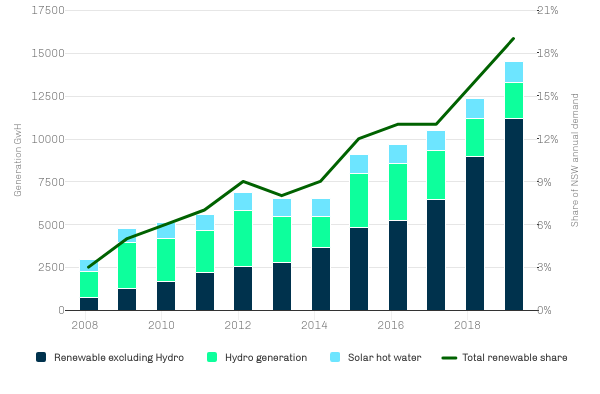
\includegraphics[width=0.95\textwidth,height=10cm]{renewable_fuel_sources_chart.png}
\caption{Renewable fuel sources [Source:
Derived from Department of the Environment and Energy, Australian Energy Statistics, Table O, June 2021]}\label{renewable}
\end{figure}

As stated in \cite{nswEnergyConsumption} the driving factors of
electricity consumption and demand forecasts can be split into two
different types: structural drivers and random drivers. Structural
drivers such as population, economic growth, electricity price,
technology adoption, energy efficiency can be estimated based on past
trends and expert judgement. On the other hand, random drivers, such as
weather, customer behavior etc, which can be modeled as probability
distributions. There are many factors that drive consumers to make
similar choices regarding electricity consumption at the same time for
example during work and school schedules. And the demand is different
during weekdays, public holidays, weekends, due to weather the use of
heating and cooling appliances, and many other societal factors, such as
whether the beach is pleasant, or the occurrence of retail promotions.

Load forecasting is usually concerned with the prediction of hourly,
daily, weekly, and annual values of the system demand and peak demand.
Such forecasts are sometimes categorized as short-term, medium-term and
long-term forecasts, depending on the time horizon. In terms of
forecasting outputs, load forecasts can also be categorized as point
forecasts (i.e., forecasts of the mean or median of the future demand
distribution), and density forecasts (providing estimates of the full
probability distributions of the possible future values of the demand).

\begin{figure}[H]
\centering
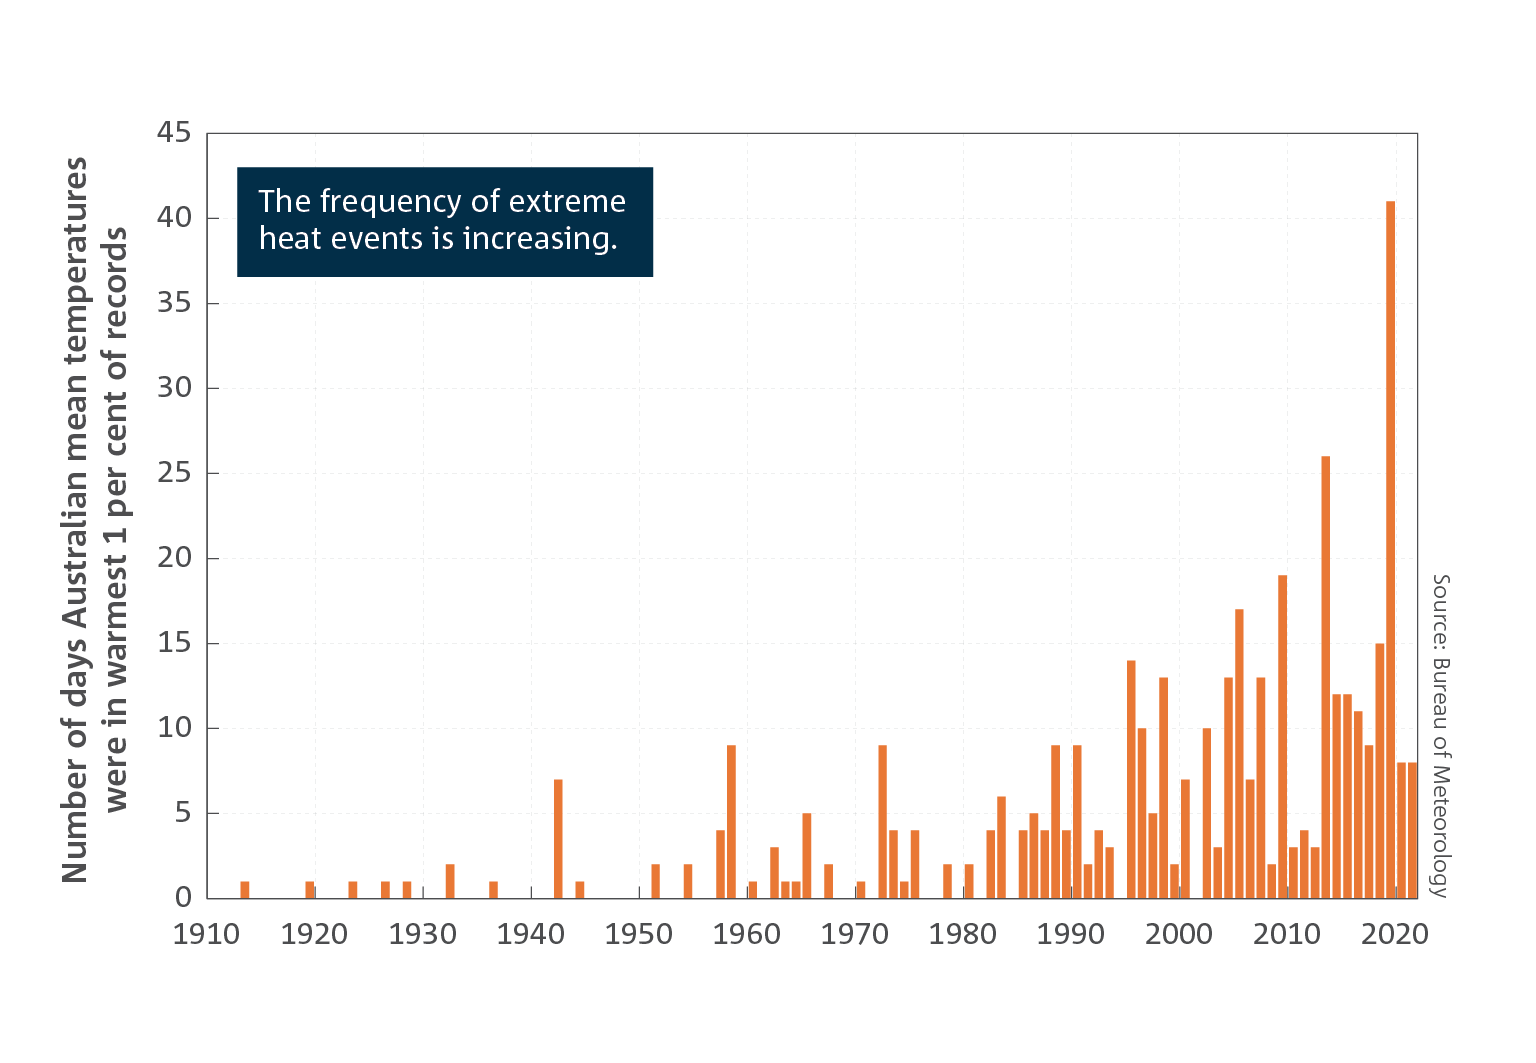
\includegraphics[width=0.95\textwidth, height=10cm]{extreme_temp__au.png}
\caption{A caption1}\label{extreme}
\end{figure}

In addition to the basic components of electricity demand forecasting,
several external factors play a significant role in refining predictions
and improving accuracy.

Temperature is a crucial factor, as it directly influences electricity
consumption patterns. Extreme temperatures, whether very hot or cold,
can lead to higher demand for heating or cooling, respectively.
Forecasts often need to account for temperature variations to predict
demand more accurately, especially during seasonal extremes or unusual
weather patterns.

As the graph in Figure \ref{extreme} shows the temperature in Australia
is rising and forecast show that it will continue to rise. According to
\cite{nswAdaptNSW} the climate of NSW is changing, with 6 of the 10
warmest years on record occurring in the past 10 years. The warmest year
on record for both average temperature and maximum temperature in NSW
was 2019, when average temperature was 1.2°C above the 1990--2009
average. Across NSW, average temperatures will continue to increase
throughout this century. By 2090, average temperature is projected to
rise by around 1.3°C under a low emissions scenario and around 4.0°C
under a high emissions scenario. So temperature is key factor while
determining the electricity demand. The usage of heating in colder
nights and cooling system during the hot days directly impacts the
demand of electricity.

Holidays and weekdays also affect electricity usage. On holidays,
electricity consumption patterns can differ significantly from regular
weekdays due to changes in work routines and social activities. For
instance, public holidays might see a decrease in commercial and
industrial electricity use, while residential usage could increase due
to family gatherings and home activities. Understanding these variations
helps in adjusting forecasts to better reflect the actual demand
patterns during such periods.

Overall, incorporating temperature data and considering holiday effects
are essential for creating more accurate and reliable electricity demand
forecasts, which in turn support better decision-making for power system
management and operational planning.

\section{Electricity Demand Forecast
Methodologies}\label{electricity-demand-forecast-methodologies}

Electricity demand or load forecasting is a well-known problem to
predict the future load based on historic information. Researchers used
both statistical and probabilistic methods to achieve high accuracy with
low errors to find the best model. They also considered this problem as
both deterministic and stochastic to include the influence of the
external factors that sways the models behaviour at different time
horizons. At high-level the problem can be classified into four
forecasting groups -- very short-term (mins to hrs), short-term (days),
medium-term (months), and long-term (years). Based on the required time
horizons we can further classify the problem into three broad solution
domains -- heuristic, statistical or econometric, and probabilistic
models. Typically, electricity consumption is influenced by two
factors---1) structural like population growth, economic condition,
electricity price, etc; and 2) non-structural or random like weather
condition e.g., air temperature, extreme heat or cold, bushfire, flood,
etc., building type e.g., multi-storey or free-standing house, and
adoption of electric vehicles and contributions of renewable energy in
the power grid, etc. Time series datasets have the unique property of
dependence on what happened on the past. Therefore, we cannot randomly
shuffle the order of the data without affecting the trends. With such
dependency simple regression technique for forecasting can randomly show
statistical significance even if there is no true correlation, and thus
suitable for real-world usage. In the following sections, we will
discuss the popular forecasting models used in the electricity demand
forecasting domain.

\section{Statistical Models/ Regression
Methods}\label{statistical-models-regression-methods}

The simplest form of forecasting is Moving Average (MA) which predicts
the future values as the average of n previous values. With a larger
window we can smooth out the noise to find the actual tend but the
forecasts will start to lag as we were to go back further and further to
calculate the average. Exponential Smoothing (ETS) eliminates this
problem by exponentially decrease the weights of the averages over time.
This prioritises more recent values over the older values, however, as
the averaging window size increases the overall trend starts to lag
again. Additionally, most real-world time series are not stationary
i.e., the change in mean or variance over time are not the same at
different observation points. Autoregressive Integrated Moving Average
(ARIMA) \cite{box1970time} extends this idea further by modelling the
dependent relationship between an observation and a set of previously
lagged observations by taking the difference of successive values many
times to make the time series stationary. This is like saying that it
will be hot tomorrow since it has been hot so far this week as the high
air temperature had not varied much. In short, the \(ARIMA(p, q, d)\)
model applies a \(d\)th order differencing on a time series and takes
the last p terms in autoregressive way and the include the last q moving
average terms to generate the forecast over a specified time horizon.
However, the ARIMA model does not consider the repeating patterns within
the time series like temperature increases in the daytime while
decreases in night or hotter summer and colder winter. Seasonal ARIMA
(SARIMA) \cite{box1970time} deals with this challenge by taking the
values of \(p\), \(q\), and \(d\) over a season period m instead of the
immediate past. Auto ARIMA \cite{Hyndman2008} scales this process by
finding the best combination of \(<p, q, d>\) automatic way. Typically,
ARIMA models and its other variants forecast very well but it's hard to
scale for large datasets and often too complex to fine tune without
significant domain expertise. The Theta Forecast
\cite{assimakopoulos2000theta} is another well performed model that uses
a parameter \(\theta\) to smooths the local curvature of a time series.
In the original implementation two theta lines are used and the final
forecast is the average of them. Later, \cite{hyndman2002forecasting}
showed that an ETS with a drift term can perform equally to the original
Theta Forecast and since then adopted to most of its later
implementations. \cite{Wang2021} highlights that although these
traditional techniques such as fuzzy linear regression, exponential
smoothing, Automatic Regressive Moving Average (ARMA) have the
advantages of algorithmic simplicity but they are not scalable to handle
large dataset and model complicated relationships.

\section{Machine Learning Methods}\label{machine-learning-methods}

Another approach is to first apply Fourier Transformation (FT) to
decompose a stationary time series (i.e., removing trends and
seasonality) from time domain to frequency domain as temporal
frequencies. Once decomposed we can then apply Fast Fourier Transform
(FFT) \cite{shannon1948mathematical} to filter out the noise and only
select the few promising frequencies to perform an Inverse Fast Fourier
Transform (IFFT) to reconstruct the time series and add back the trend
and seasonality. Due to its unique properties FFT is a versatile and
fast generic tool to identify trends and noise filtering in time series
and therefore often used as to establish a baseline forecast. A more
recent and very popular Generalised Additive Model (GAM) for regression
technique is \emph{Prophet} \cite{taylor2017facebook}. It is designed to
optimally handle business forecasting tasks featuring time series
captures at the hourly, daily, or weekly level with ideally at least a
full year of historical data. It can also handle missing data and
outliers, strong seasonality effects occurring daily, weekly, yearly,
holidays and other special one-time events that do not necessarily
follow the seasonality patterns. These unique properties make it very
suitable for both short-term and mid-term electricity forecasting as we
will discuss the \emph{Prophet} model in greater details in following
subsection. Instead of finding a single point forecast from a time
series using statistical methods discussed in the previous subsection,
we can also apply probabilistic methods like probabilistic regression or
other machine learning models. In the simplest form to cast a time
series forecasting as regression we need to first convert the
observations i.e., samples as 